%% tags: squiggly snake snakes decoration scope relativeToScope directed network arrow parbox
\documentclass[tikz,border=2]{standalone}
\usetikzlibrary{decorations.pathmorphing,shadows,arrows,shapes,positioning,calc,backgrounds,fit,automata}
\begin{document}
%%%%%%%%%%%%%%%%%%%%%%%%%%%%%%%%%%%%%%%
% Define the layers to draw the diagram
\pgfdeclarelayer{bg}
\pgfsetlayers{bg,main}
%%%%%%%%%%%%%%%%%%%%%%%%%%%%%%%%%%%%%%%
% colors
\definecolor{myBlue}{HTML}{0060AD}
\definecolor{myRed}{HTML}{DD181F}
%%%%%%%%%%%%%%%%%%%%%%%%%%%%%%%%%%%%%%%

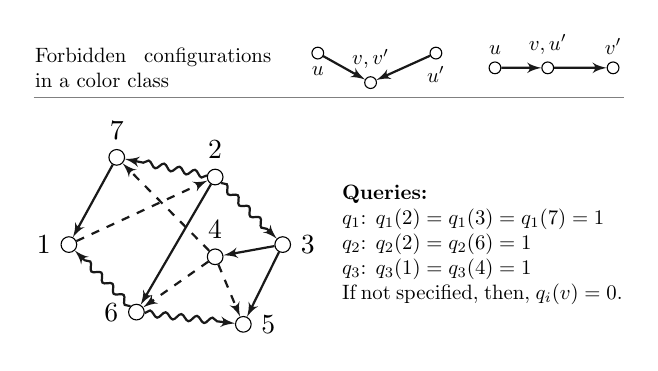
\begin{tikzpicture}
[scale=1,transform shape,node distance=1cm,
vertex/.style={shape=circle,inner sep=2pt,draw},
anc/.style={inner sep=0pt},
%
c1/.style={},
c2/.style={decorate,decoration={snake,amplitude=.4mm,segment
length=2mm,post length=1.5mm,pre length=0mm}},
%%decoration={snake,amplitude=.4mm,segment length=2mm, post length=0mm,pre
%%length=0mm},
c3/.style={dashed},
%
myedge/.style={thick,>=latex', shorten >=.0pt, black!90, shorten <=.0pt}]
%
\begin{scope}[local bounding box=example]
\node (v1) [vertex,label=left:$1$] at (0,0) {};
\node (v2) [vertex,above right=of v1,shift={(1,0)},label=above:$2$] {};
\node (v3) [vertex,below right=of v2,shift={(0,0)},label=right:$3$] {};
\node (v4) [vertex,below=of v2,shift={(0,.2)},label=above:$4$] {};
\node (v5) [vertex,below=of v3,shift={(-.5,.2)},label=right:$5$] {};
\node (v6) [vertex,below right=of v1,label=left:$6$] {};
\node (v7) [vertex,above right=of v1,shift={(-.25,.25)},,label=above:$7$] {};
%% \node [above left=of v1] {$G$};
%
\draw[myedge,c3,->] (v1) -- (v2);
\draw[myedge,c2,->] (v6) -- (v1);
\draw[myedge,c1,<-] (v1) -- (v7);
%
\draw[myedge,c2,->] (v2) -- (v3);
\draw[myedge,c1,->] (v2) -- (v6);
\draw[myedge,c2,->] (v2) -- (v7);
%
\draw[myedge,c1,->] (v3) -- (v4);
\draw[myedge,c1,->] (v3) -- (v5);
%
\draw[myedge,c3,->] (v4) -- (v5);
\draw[myedge,c3,->] (v4) -- (v6);
\draw[myedge,c3,->] (v4) -- (v7);
%
\draw[myedge,c2,->] (v6) -- (v5);
\end{scope}
%
\begin{scope}[scale=.75,transform shape, shift={(7,0)}]
\newcommand{\parnode}[1]{\parbox{4.75cm}{#1}}
\node{\parnode{
\textbf{Queries:}\\
$q_1$: $q_1(2)=q_1(3)=q_1(7)=1$\\
$q_2$: $q_2(2)=q_2(6)=1$\\
$q_3$: $q_3(1)=q_3(4)=1$\\
If not specified, then, $q_i(v)=0$.
}};
\end{scope}
%%
\begin{scope}[anchor=west,scale=.75,transform shape, shift={($(example.north
    west)+(0,.75)$)}]
\node{\parbox{4cm}{{Forbidden configurations in a color class}}};
\draw[black!50] (.1,-.5) -- ++(10,0);
\begin{scope}[scale=1,transform shape, shift={(5.7,-.25)}]
\node (v1) [vertex,label=above:{$v,v'$}] at (0,0) {};
\node (v2) [vertex,label=below:$u$,shift={(-1,.5)}] at (v1) {};
\node (v3) [vertex,label=below:$u'$,shift={(1,.5)}] at (v1) {};
\draw[myedge,<-] (v1) -- (v2);
\draw[myedge,<-] (v1) -- (v3);
\end{scope}
%%
\begin{scope}[scale=1,transform shape, shift={(8.7,-.25)}]
\node (v1) [vertex,label=above:{$v,u'$}] at (0,.25) {};
\node (v2) [vertex,label=above:$u$,shift={(-1,0)}] at (v1) {};
\node (v3) [vertex,label=above:$v'$,shift={(1,0)}] at (v1) {};
\draw[myedge,<-] (v1) -- (v2);
\draw[myedge,->] (v1) -- (v3);
\end{scope}
\end{scope}
\end{tikzpicture}
\end{document}
